\chapter{Data For ML: Text Data}

\section{Terminologies \cite{nlp-1, chatgpt, ir-1}}
\begin{customTableWrapper}{1}
\begin{table}[h!]
    \centering
    \begin{tabular}{| m{2cm} | m{6cm} | m{6cm} |}
        \hline
        \customTableHeaderColor
        \textbf{Term} & \textbf{Definition} & \textbf{Example} \\
        \hline
        \textbf{(Document) Collections} aka \textbf{Corpus} & \vspace{0.2cm}\begin{enumerate}
            \item A group of documents or texts gathered together, often around a specific theme, topic, or source. 
            
            \item Collections can be subsets within a larger corpus.

            \item group of documents over which we perform retrieval \cite{ir-1}
        \end{enumerate} & A collection of scientific articles on climate change, or a collection of user reviews from a specific website. \\
        \hline
        
        \textbf{Documents} & \vspace{0.3cm}\begin{enumerate}
            \item Individual pieces of text within a corpus or a collection. They are the smallest unit of analysis and can vary in length and format.
            
            \item whatever units we have decided to build a retrieval system over. \cite{ir-1}
        \end{enumerate} & A single news article, a research paper, a blog post, or a book chapter. \\
        \hline
        
    \end{tabular}
\end{table}
\end{customTableWrapper}

\section{Herdan’s Law ( $\dabs{V} = kN^{\beta}$ ) \cite{nlp-1}} \label{Herdan’s Law}

\[
    \dabs{V} = kN^{\beta} \hfill (0 < \beta < 1 \text{ and } k > 0)
\]

\begin{enumerate}
    \item The larger the corpora we look at, the more word types we find.
    \item value of $\beta$ depends on the corpus size and the genre
\end{enumerate}

\section{Datasheet/ Data statement}\label{Datasheet/ Data statement}

A datasheet specifies properties of a dataset like:
\begin{customTableWrapper}{1.3}
\begin{table}[h]
    \centering
    \begin{tabular}{|m{3.5cm}|m{11.5cm}|}
        \hline
        
        \textbf{Motivation} & Why was the corpus collected, by whom, and who funded it?  \\ 
        \hline
         
         \textbf{Situation} & When and in what situation was the text written/spoken? For example, was there a task? Was the language originally spoken conversation, edited text, social media communication, monologue vs. dialogue? \\
         \hline
         
        \textbf{Language variety} & What language (including dialect/region) was the corpus in? \\
        \hline
        
        \textbf{Speaker demographics} & What was, e.g., the age or gender of the text’s authors? \\
        \hline
        
        \textbf{Collection process} & How big is the data? If it is a subsample how was it sampled? Was the data collected with consent? How was the data pre-processed, and what metadata is available? \\
        \hline

        \textbf{Annotation process} & What are the annotations, what are the demographics of the annotators, how were they trained, how was the data annotated? \\ 
        \hline

        \textbf{Distribution} & Are there copyright or other intellectual property restrictions?\\
        \hline
        
    \end{tabular}
\end{table}
\end{customTableWrapper}

\section{Term-document incidence matrix \cite{ir-1}}\label{Term-document incidence matrix}

Matrix element $(t, d)$ is $1$ if the play in column $d$ contains the word in row $t$, and is $0$ otherwise.

Example:
\begin{table}[h]
    \centering
    \begin{tabular}{l c c c c c c c c}
         & doc1 & doc2 & doc3 & doc4 & doc5 & doc6 & $\cdots$ & docN \\
        term1 & 1 & 0 & 1 & 1 & 1 & 0 & $\cdots$ & 1 \\ 
        term2 & 1 & 1 & 0 & 1 & 0 & 0 & $\cdots$ & 0 \\ 
        $\vdots$ & $\vdots$ & $\vdots$ & $\vdots$ & $\vdots$ & $\vdots$ & $\vdots$ & $\ddots$ & $\vdots$ \\
        termV & 0 & 0 & 1 & 0 & 1 & 1 & $\cdots$ & 0 \\ 
    \end{tabular}
    \caption{Term-document incidence matrix - Example}
\end{table}



\section{Term-document matrix \cite{nlp-1}}\label{Term-document matrix}

\begin{enumerate}
    \item In a term-document matrix, each row represents a word in the vocabulary and each column represents a document from some collection of documents.
    
    \item The term-document matrix was first defined as part of the \textbf{vector space model}\indexlabel{vector space model} of information retrieval. In this model, a document is represented as a count vector.

    \item in term-document matrices, the vectors representing each document would have dimensionality $\dabs{V}$ (vocabulary size).

    \item Two documents that are similar will tend to have similar words, and if two documents have similar words their column vectors will tend to be similar.

    \item documents can be represented as vectors in a vector space. A \textbf{vector space} (SEE: \fullref{Vector Spaces}) is a collection of vectors, characterized by their dimension.
\end{enumerate}

Example:
\begin{table}[h]
    \centering
    \begin{tabular}{l c c c c c c c c}
         & doc1 & doc2 & doc3 & doc4 & doc5 & doc6 & $\cdots$ & docN \\
        term1 & 4 & 0 & 2 & 0 & 154 & 0 & $\cdots$ & 10 \\ 
        term2 & 0 & 114 & 5 & 1 & 0 & 89 & $\cdots$ & 0 \\ 
        $\vdots$ & $\vdots$ & $\vdots$ & $\vdots$ & $\vdots$ & $\vdots$ & $\vdots$ & $\ddots$ & $\vdots$ \\
        termV & 87 & 41 & 0 & 0 & 0 & 0 & $\cdots$ & 35 \\ 
    \end{tabular}
    \caption{Term-document matrix - Example}
\end{table}


\section{Co-occurrence matrix/ term-term matrix/ word-word matrix/ term-context matrix \cite{nlp-1}}\label{Co-occurrence matrix/ term-term matrix/ word-word matrix/ term-context matrix}

\begin{enumerate}
    \item columns are labeled by words rather than documents. 
    
    \item Dimensionality $\dabs{V}\times\dabs{V}$ and each cell records the number of times the row (target) word and the column (context) word co-occur in some context in some training corpus.

    \item The context could be the document, in which case the cell represents the number of times the two words appear in the same document.

    \item It is most common, however, to use smaller contexts, generally a window around the word, for example of $4$ words to the left and $4$ words to the right, in which case the cell represents the number of times (in some training corpus) the column word occurs in such a $\pm 4$ word window around the row word.

    \item Since most of the entries of the matrix are zero these are \textbf{sparse vector representations}.
\end{enumerate}

Example:
\begin{table}[h]
    \centering
    \begin{tabular}{l c c c c c c c c}
         & term1 & term2 & $\cdots$ & termV \\
        term1 & 4 & 0 & $\cdots$ & 10 \\ 
        term2 & 0 & 114 & $\cdots$ & 0 \\ 
        $\vdots$ & $\vdots$ & $\vdots$ & $\ddots$ & $\vdots$ \\
        termV & 87 & 41 & $\cdots$ & 35 \\ 
    \end{tabular}
    \caption{Co-occurrence matrix/ term-term matrix/ word-word matrix/ term-context matrix - Example}
\end{table}

\section{Term Frequency ( $\rcmdXtf_{t,d}$ ) \cite{nlp-1}} \label{Term Frequency}

the frequency of the word/ term $t$ in the document $d$.
\[
    \rcmdXtf_{t,d} = \rcmdXcount(t,d) \hfill \text{(raw count)}
\]
\[
    \rcmdXtf_{t,d} = \begin{dcases}
        1 + \log_{10}(\rcmdXcount(t,d)) & \text{ if } \rcmdXcount(t,d) > 0\\
        0 & \text{ otherwise}
    \end{dcases} \hfill \text{(Squashed raw frequency)}
\]


\section{Document Frequency ( $\rcmdXdf_t$ ) \cite{nlp-1}}\label{Document Frequency}

\begin{enumerate}
    \item The second factor in tf-idf is used to give a higher weight to words that occur only in a few documents.

    \item Terms that are limited to a few documents are useful for discriminating those documents from the rest of the collection; terms that occur frequently across entire collection aren't as helpful.

    \item The document frequency $\rcmdXdf_t$ of a word/ term $t$ is the number of documents it occurs in.
\end{enumerate}

\section{Collection frequency \cite{nlp-1}}\label{Collection frequency}
total number of times the word appears in the whole collection in any document.


\section{inverse document frequency/ idf term weight ( $\rcmdXidf_t$ )}\label{inverse document frequency/ idf term weight}
\[
    \rcmdXidf_t = \displaystyle\dfrac{N}{\rcmdXdf_t} \hfill \text{(raw frequancies)}
\]
\[
    \rcmdXidf_t = \log_{10} \left(\displaystyle\dfrac{N}{\rcmdXdf_t} \right) \hfill \text{(squashed)}
\]

Where,
\begin{enumerate}
    \item $N$ is the total number of documents in the collection
    \item $dft$ is the number of documents in which term t occurs.
\end{enumerate}

\vspace{0.2cm}
\textbf{Note}:
\begin{enumerate}
    \item The fewer documents in which a term occurs, the higher this weight.

    \item The lowest weight of $1$ is assigned to terms that occur in all the documents.

    
\end{enumerate}


\section{tf-idf weighted value ( $w_{t,d}$ ) \cite{nlp-1}}\label{tf-idf weighted value: formula}
\[
    w_{t,d} = \rcmdXtf_{t,d} \times\rcmdXidf_t
\]

\section{Inverted Index/ inverted file \cite{ir-1}}\label{Inverted Index/ inverted file}

\begin{figure}[h]
    \centering
    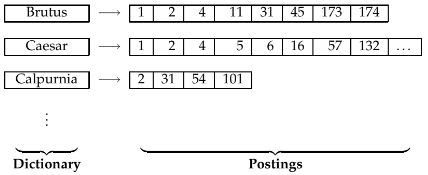
\includegraphics[width=\linewidth, height=2.5cm, keepaspectratio]{Pictures/info-retrieval/inverted-index.png}
    \caption{Inverted Index/ inverted file - example}
\end{figure}

\begin{enumerate}
    \item The name is actually redundant: an index always maps back from terms to the parts of a document where they occur. 
    
    \item \textbf{Inverted index}, or sometimes \textbf{inverted file}, has become the standard term in information retrieval.    
\end{enumerate}


\noindent \textbf{Steps}:
\begin{enumerate}
    \item \textbf{Collect} the documents to be indexed:\\
    \fbox{Friends, Romans, countrymen.} \fbox{So let it be with Caesar} $\cdots$

    \vspace{0.5cm}
    \item \textbf{Tokenize} the text, turning each document into a list of tokens:\\
    \fbox{Friends} \fbox{Romans} \fbox{countrymen} \fbox{So} \fbox{let} \fbox{it} \fbox{be} \fbox{with} \fbox{Caesar} $\cdots$

    \vspace{0.5cm}
    \item Do linguistic \textbf{preprocessing}, producing a list of normalized tokens, which are the indexing terms:\\
    \fbox{friend} \fbox{roman} \fbox{countryman} \fbox{so} $\cdots$

    \vspace{0.5cm}
    \item \textbf{Index} the documents that each term occurs in by creating an inverted index, consisting of a dictionary and postings.
\end{enumerate}


\noindent\textbf{Note}:
\begin{enumerate}
    \item each document has a \textbf{unique serial number}, known as the \textbf{document identifier}\indexlabel{docID: document identifier} ($docID$).\\
    During index construction, we can simply assign \textbf{successive integers} to each new document when it is first encountered.\\
    The input to indexing is a list of normalized tokens for each document, which we can equally think of as a list of pairs of term and $docID$.

    \item The core indexing step is \textbf{sorting} this list so that the terms are alphabetical.

    \item Multiple occurrences of the same term from the same document are then merged.

    \item Instances of the same term are then grouped, and the result is split into a dictionary and postings.

    \item Since a term generally occurs in a number of documents, this data organization already reduces the storage requirements of the index. 
    
    \item The dictionary also records some statistics, such as the number of documents which contain each term (the \textbf{document frequency}, which is here also the length of each postings list).

    \item The postings are secondarily sorted by $docID$.\\
    This provides the basis for efficient query processing.

    \item This inverted index structure is essentially without rivals as the most efficient structure for supporting ad hoc text search.

    \item In the resulting index, we pay for storage of both the dictionary and the postings lists.\\
    The latter are much larger, but the dictionary is commonly kept in \textbf{memory}, while postings lists are normally kept on \textbf{disk}, so the size of each is important.

    \item A fixed length array would be wasteful as some words occur in many documents, and others in very few. For an in-memory postings list, two good alternatives are \textbf{singly linked lists} or \textbf{variable length arrays}.
    \begin{enumerate}
        \item \textbf{Singly linked lists} allow cheap insertion of documents into postings lists, which require additional pointers.

        \item \textbf{Variable length arrays} win in space requirements by avoiding the overhead for pointers and in time requirements because their use of \textbf{contiguous memory} increases speed on modern processors with memory caches.\\
        Extra pointers can in practice be encoded into the lists as offsets.\\
        If updates are relatively infrequent, variable length arrays will be more compact and faster to traverse.

        \item We can also use a hybrid scheme with a linked list of fixed length arrays for each term.\\
        When postings lists are stored on disk, they are stored (perhaps compressed) as a contiguous run of postings without explicit pointers, so as to minimize the size of the postings list and the number of disk seeks to read a postings list into memory.
    \end{enumerate}

    
\end{enumerate}

\noindent \textbf{Example}:
\begin{table}[h]
    \begin{minipage}[t]{.45\linewidth}
        \textbf{Doc1}\\
        I did enact Julius Caesar: I was killed i’ the Capitol; Brutus killed me.
    \end{minipage}
    \hfill
    \begin{minipage}[t]{.45\linewidth}
        \textbf{Doc2}\\
        So let it be with Caesar. The noble Brutus hath told you Caesar was ambitious:
    \end{minipage}
    \caption{Inverted Index - Step 1}
\end{table}

\begin{table}[h]
    \begin{minipage}[t]{0.25\linewidth}
        \begin{table}[H]
            \centering
            \begin{tabular}{l r}
                \textbf{term} & \textbf{docID} \\
                I & 1 \\
                did & 1 \\
                enact & 1 \\
                $\vdots$ & $\vdots$ \\
                was & 2 \\
                ambitious & 2 \\
            \end{tabular}
            \caption{Inverted Index - Step 2}
        \end{table}
    \end{minipage}
    \hfill
    \begin{minipage}[t]{0.25\linewidth}
        \begin{table}[H]
            \centering
            \begin{tabular}{l r}
                \textbf{term} & \textbf{docID} \\
                ambitious & 2 \\
                be & 2 \\
                brutus & 1 \\
                $\vdots$ & $\vdots$ \\
                was & 2 \\
                with & 2 \\
            \end{tabular}
            \caption{Inverted Index - Step 3}
        \end{table}
    \end{minipage}
    \hfill
    \begin{minipage}[t]{0.4\linewidth}
        \begin{table}[H]
            \centering
            \begin{tabular}{l l c l}
                \textbf{term} & \textbf{doc. freq.} & $\to$ & \textbf{postings lists} \\
                \fbox{ambitious} & \fbox{1} & $\to$ & \fbox{2} \\
                \fbox{be} & \fbox{1} & $\to$ & \fbox{2} \\
                \fbox{brutus} & \fbox{2} & $\to$ & \fbox{1} $\to$ \fbox{2} \\
                $\vdots$ & $\vdots$ \\
                \fbox{was} & \fbox{2} & $\to$ & \fbox{1} $\to$ \fbox{2} \\
                \fbox{with} & \fbox{1} & $\to$ & \fbox{2} \\
            \end{tabular}
            \caption{Inverted Index - Step 4}
        \end{table}
    \end{minipage}
\end{table}





























